\chapter{The LHC and CMS Machine}
In this chapter, the working and the design parameters of Large Hadron Collider (LHC) and its one of main purpose detector is briefly described.

\section{The Large Hadron Collider}
The famous quote ``history repeats itself" applies well to the \acrfull{hep}. The starting point of experimental high energy physics is the Rutherford $\alpha$-particle scattering, and even now we are doing the same thing just the method changed from ``natural accelerator" to the ``man-made" accelerator that can accelerate particles with the velocity close to the speed of light. The design and working of accelerator changed a lot over a period of time in going from MeV to GeV and in the TeV range. Now, these machines are not only used in \acrshort{hep} experiments, but extends its arena to treat human beings like cancer therapy, radioisotope production, also to the industry for uses like material processing, sterilisation, security scan, water treatment, and many more. 

The \acrfull{lhc} is  a hadron collider which can accelerate the two proton beams in opposite direction with maximum of 14 TeV energy in a 26.6 km long tunnel which is about 100 m underground.
The \acrfull{lhc} is the latest and most-\todo[fancyline]{Find better word}powerful accelerator everbuilt. It is a proton-proton collider built to improve our understanding of fundamental physics. It started on 21$^{st}$ October 2008. It is built on in the same tunnel where there was Large Electron Positron (LEP) collider, that collides electrons and positrons. LEP collaboration decided to switch to hadron collider because of following advantages:
\begin{itemize}
    \item Hadron collider can reach a higher centre of mass (COM) energy, because of much lower synchrotron radiation emitted by hadrons as compared to electrons. Synchrotron radiation loss is directory proportional to $(Energy/mass)^4$.
    \item As hadrons are composit particles so it allows us to scan over wide range of energy.
\end{itemize}

The CERN accelerator complex is shown in Fig. \ref{fig:CERN-accelerator-complex}.  The acceleration of protons are done in several steps. \todo[fancyline]{Write again the accelerator chain information.} They are:
\begin{itemize}
    \item Grab proton source: The source of proton is Duoplasmatron\footnote{It strips electron from hydrogen gas and creates a plasma of protons, electrons and molecular ions. This plasma expands towards the extraction electrodes and a protom beam is formed}\cite{LHC-tdr-vol3}. This feed protons to LINAC2.
    \item LINAC2 (Linear accelerator-2): It is the starting point for the protons used in the LHC accelerator complex. Here, protons reaches to an energy of 50 $MeV$ using the radiofrequency cavities where it also gains 5\% in mass. It feeds to the Proton Synchtron Booster (PSB).
    \item PSB: It takes 50 $MeV$ protons beams from LINAC2 and accelerates it to 1.4 $GeV$ for the injection into Proton Synchtron (PS).
    \item PS: It is one of key component in the LHC accelerator complex. It increases the energy of protons upto 25 $GeV$.
    \item Super Proton Synchtron (SPS): It has a circumference of 7 $km$ where protons are accelerated to an energy of 450 $GeV$. Then via two transmission line protons are then injected into LHC ring.
    \item LHC: It grabs two proton beams from SPS which is injected into opposite direction in parallel pipes. In LHC proton beams can be accelerated upto 7 $TeV$.
\end{itemize}
\begin{figure}[!ht]
  % \centering
  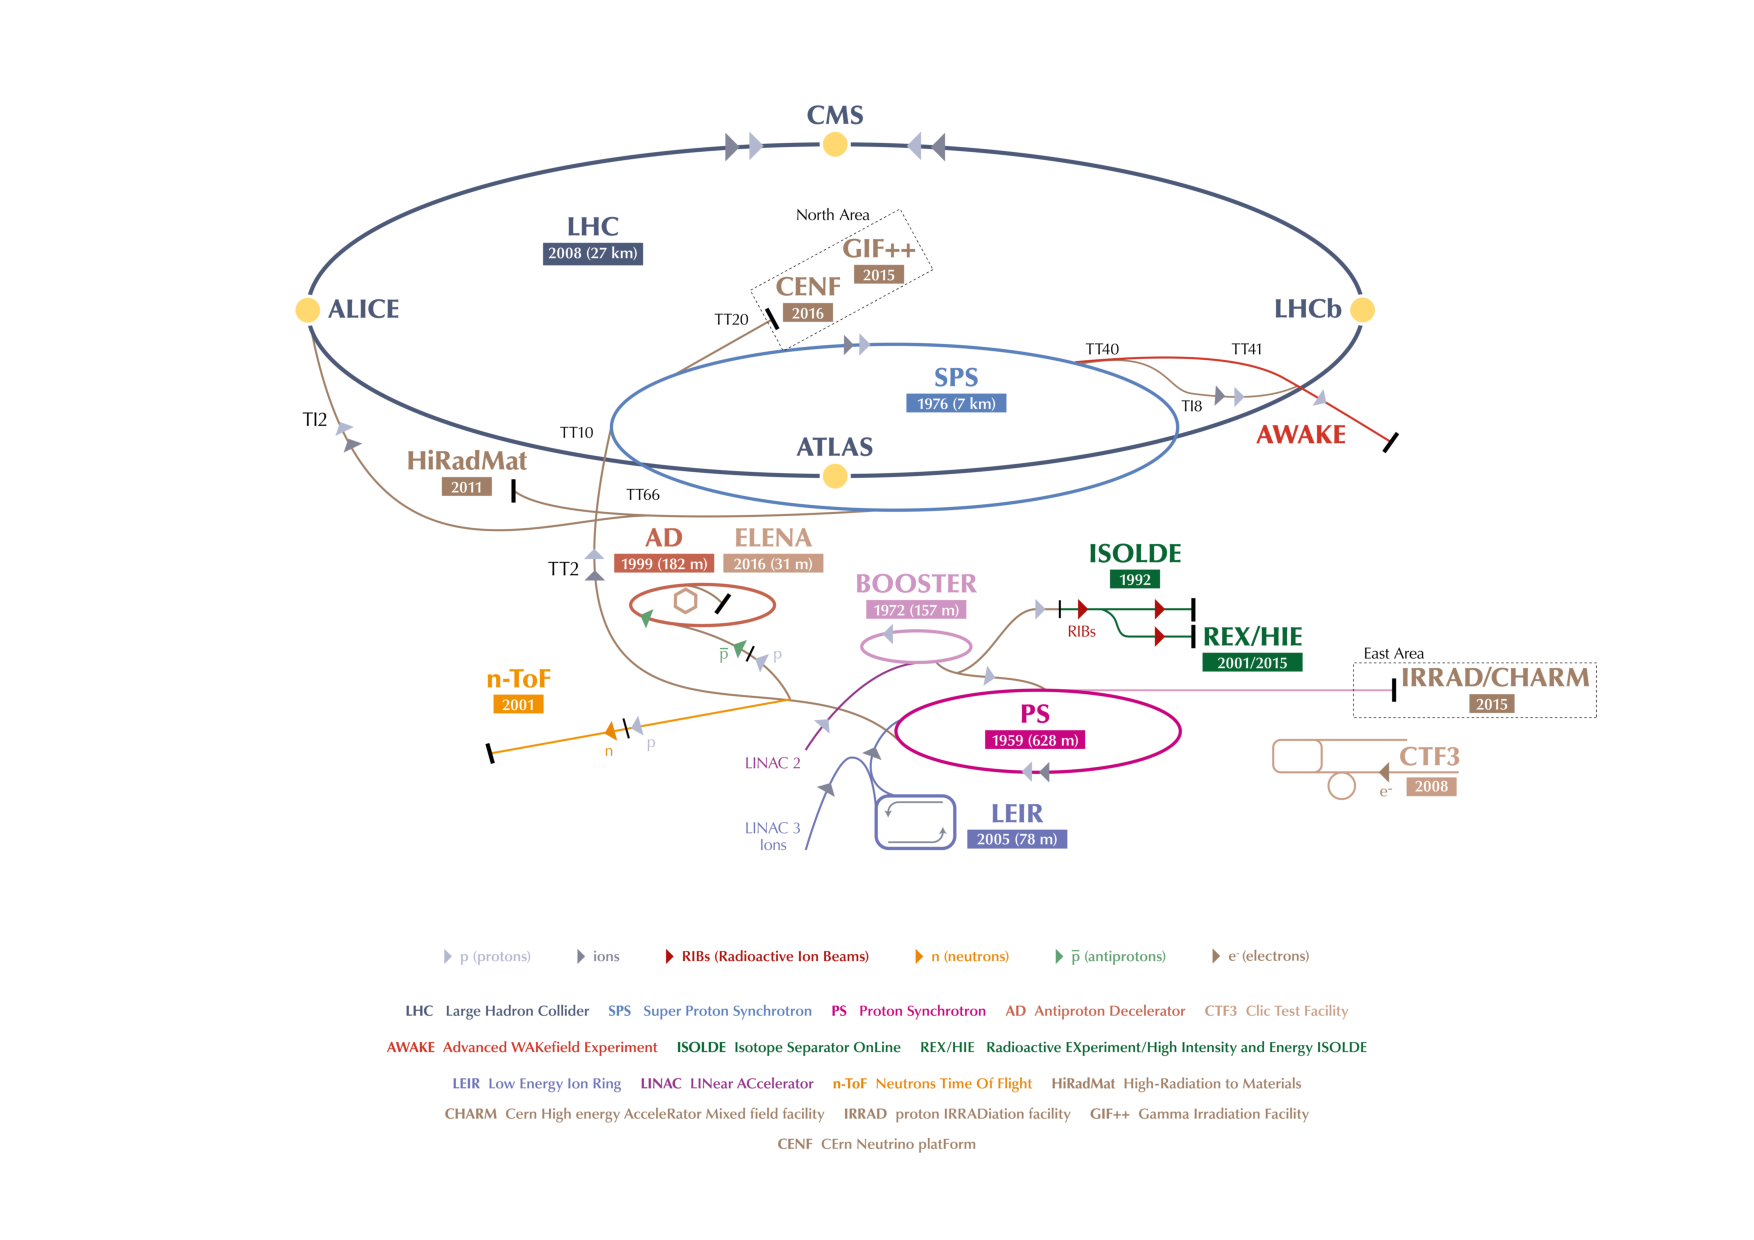
\includegraphics[width=16cm,height=18cm]{figures/CERN_Accelerator_Complex-v2016.pdf}
  \caption{The LHC is the last ring (dark blue line) in a complex chain of particle accelerators. The smaller machines are used in a chain to help boost the particles to their final energies and provide beams to a whole set of smaller experiments, which also aim to uncover the mysteries of the Universe.\todo[inline]{Update the caption.} \cite{Fig-CERN-accelerator-complex}}
  \label{fig:CERN-accelerator-complex}
\end{figure}



The interaction in HEP experiments are characterized by mainly the center of mass energy along with type and number of particles.


Below table is taken from \cite{Schoerner-Sadenius2015, LHC-parameters-2016, LHC-tdr-vol1}.


\begin{table}
\centering
\begin{tabular}[!ht]{l c}
\hline
{\bf Parameters} & {\bf Value} \\
\hline
Circumference of LHC ring   &   26658.883 m \\
\hline
Maximum dipole magnetic field   & 8.33 T \\
Dipole operating temperature    & 1.9 K \\
\hline
Maximum stored energy per beam (nominal) &   362 MJ \\
Maximum stored energy per beam  (2012) &   143 MJ \\
Maximum stored energy per beam  (2016) &   266 MJ \\
\hline
Beam energy at Injection    & 450 GeV \\
Beam energy at collision (nominal) &    7 TeV \\
Beam energy at collision (2012)     &   4 TeV \\
Beam energy at collision (2016)     &   6.5 TeV \\
\hline
Maximum instantaneous luminosity (nominal)  &   $10^{34}$ cm$^-2$ s$^{-1}$ \\
Maximum instantaneous luminosity (2012)     &   $7.7 \times 10^{33}$ cm$^-2$ s$^{-1}$ \\
Maximum instantaneous luminosity (2016)     &   $1.4 \times 10^{34}$ cm$^-2$ s$^{-1}$ \\
\hline
Number of bunches per proton beam (nominal) &   2808 \\
Number of bunches per proton beam (2012)    &   1380 \\
Number of bunches per proton beam (2016)    &   2076 \\
Maximum number of protons per bunch         &   $1.6 \times 10^{11}$ \\
\hline
Protons/bunch (average at start of collision) (nominal)   &   $1.15 \times 10^{11}$ \\
Protons/bunch (average at start of collision) (2012)  &   $1.5 \times 10^{11}$ \\
Protons/bunch (average at start of collision) (2016)  &   $1.1 \times 10^{11}$ \\
\hline
Bunch collision frequency (nominal)         &   40 MHz  \\
Bunch collision frequency (2012)            &   20 MHz  \\
Bunch collision frequency (2016)            &   40 MHz  \\
\hline
Bunch length (at injection)   &   1.7 ns \\
Bunch length (at collision)   &   1.05 ns \\
Energy spread (at injection)   &   1.9$\times 10^{-3}$ \\
Energy spread (at collision)   &   0.45$\times 10^{-3}$  \\
\hline
Half crossing angle  (nominal)   & 143 $\mu rad$ \\
Half crossing angle  (2012)   & 146 $\mu rad$ \\
Half crossing angle  (2016)   & 185 $\mu rad$ \\
\hline
$\beta *$  (nominal) &   0.55 m\\
$\beta *$   (2012)&   0.6 m\\
$\beta *$   (2016)&   0.4 m\\
\hline
RMS beam size at IP1 \& IP5 &   17 $\mu m$ \\
RMS beam size at IP2 \& IP8 &   71 $\mu m$ \\
\hline
$\epsilon_n$(transverse emittance, rms, normalized) (at injection) &   3.5 $\mu$m\\
$\epsilon_n$(transverse emittance, rms, normalized) (at collision point) &   3.75 $\mu$m\\
\hline
total longitudinal emittance (at injection) & 1.0 eVs \\
total longitudinal emittance (at collision) & 2.5 eVs \\

\hline
Average mean pile-up (nominal) &   \begin{minipage}{5cm} \todo[inline]{Add pile-up for 2012 and 2016}\end{minipage} \\
Average mean pile-up (2012) &    ?? \\
Average mean pile-up (2016) &    ?? \\
\hline
Energy loss per turn at 14 TeV              &   7 keV   \\
Energy loss per turn for electrons          &  \begin{minipage}{5cm}  \todo[inline]{add synchtron energy loss for electrons} \end{minipage}     \\
\end{tabular}
\caption{LHC technical parameters for proton-proton collisions: nominal, 2012 and 2016 values.\cite{Bruce2016}.}
\label{table:LHC-parameters}
\end{table}

\begin{figure}[!ht]
  % \centering
  \includegraphics[width=12cm,height=10cm]{figures/lumi-proj-2016-final-v2}
  \caption{The integrated luminosity of the LHC with proton-proton collisions in 2016 compared to previous years. Luminosity is a measure of a collider’s efficiency and is proportional to the number of collisions. The integrated luminosity achieved by the LHC in 2016 far surpassed expectations and is double that achieved at a lower energy in 2012. (Image : CERN)\todo[inline]{Update the caption.}} 
  \label{fig:lumi-proj-2016-final-v2}
\end{figure}

\subsection{LHC Requirements}
For a collider like LHC the figure of merit   

    is luminosity. The luminosity is proportional tot he number of events per second so it shold be maximized. Luminosity is defined as:
\begin{equation}
    L = \frac{k_bN_b^2f_{rev}\gamma}{4 \pi \epsilon_n \beta^*}
\end{equation}
where,\\
\hspace{2cm}$k_b$ is the number of bunches per ring,\\
\hspace{2cm}$N_b$ is the number of protons per bunch,\\
\hspace{2cm}$f_{rev}$ the revolution frequency,\\
\hspace{2cm}$\epsilon_n$ is the normalized RMS transverse beam emittance (same in both )\\
\hspace{2cm}$\beta^*$ is the beta-function at the interaction point\\

Based on the definition of luminosity, to maximize we have to do following\todo{Remove plag below}:
\begin{itemize}
    \item The beam emmitence, $\epsilon_n$, should be low.
    \item The total intensity $k_b.N_b$ is limited by the thermal energy produced by synchtron radiation, which should be efficiently absorbed by the cryogenic system.
    \item The beam-beam effect is proportional to the transverse beam brightness $N_b/\epsilon_n$ - causing a spread in betatron tunes (``footprint") when the beams are colliding has to be kept below a certain limit;
    \item the space-charge limit in the injectors, which also scales with $N_b/\epsilon_n$.
\end{itemize}